\chapter{Results: Sensitivity Analysis}
In this chapter, DYMOND and \Cyclus are used to conduct 
sensitivity analysis studies of the 
EG01-30 \gls{NFC} transition scenario. 
Dakota-\Cyclus (\texttt{dcwrapper}) 
and Dakota-DYMOND coupling (\texttt{ddwrapper})
are used for 
one-at-a-time sensitivity analysis (SA), synergistic 
SA, and global SA. 
This chapter is broken into five sections: 
\begin{enumerate}
    \item Transition Scenario Specifications 
    \item Sensitivity Analysis Evaluation Metrics 
    \item One-at-a-time \gls{SA}
    \item Synergistic \gls{SA}
    \item Global \gls{SA}
    \item Main Takeaways 
\end{enumerate}

\section{Transition Scenario Specification}
% improve this section 
A EG01-30 transition scenario is used for 
both DYMOND and \Cyclus sensitivity analysis. 
Slight differences lie in the values of some input variables. 

\subsection{DYMOND}
The specifications of the EG01-30 transition scenario used in DYMOND 
is described in the DYMOND OECD benchmark transition 
scenario presented at the 17th Meeting of Expert Group on Advanced 
Fuel Cycle Scenarios in France in 2017 
\cite{oecd_nuclear_energy_agency_wpfc_nodate}. 
The OECD benchmark scenario is based on the EG01-30 transition scenario 
in which a \gls{PWR} fleet is transitioned to
a mixed fleet of \gls{MOX} \glspl{PWR} and \glspl{SFR}. 
Table \ref{tab:dymondinputs} describe high-level OECD benchmark transition 
scenario specifications. 

\begin{table}[H]
    \caption{OECD Benchmark Transition Scenario
	Specifications \cite{oecd_nuclear_energy_agency_wpfc_nodate}}
	\label{tab:dymondinputs}
    \scriptsize
    \begin{tabularx}{\textwidth}{LL}
    \hline
                               \textbf{Input Parameter}            & \textbf{Value}            \\ \hline
    Demand driving commodity   & Power              \\
                               Demand equation {[}TWhe/y{]}   & 430        \\
                               Transition Start Date [Year] & 80\\ 
                               Fleet share ratio [\%] & \gls{MOX} \gls{PWR}: 15\%, \gls{SFR}: 85\%\\ \hline
    \end{tabularx}%
    \end{table}

\subsection{\Cyclus}
\Cyclus transition scenario sensitivity analysis uses 
the linearly increasing power demand EG01-30 transition scenario 
(described in the Section \ref{sec:eg01-30}).  
Figure \ref{fig:30flow} shows the facility and mass flow 
for this transition scenario in \Cyclus. 
Tables \ref{tab:bestinputs} and \ref{tab:facinputs}
shows the input parameters for \deploy and 
in the transition scenario. 
The \texttt{reactor} facility used in the \Cyclus simulation 
is a recipe reactor; it accepts a fresh fuel recipe and outputs 
a spent fuel recipe. 
The recipes used for the \gls{LWR}, \gls{MOX} \gls{LWR}, and 
\gls{SFR} are based on recipes generated by VISION 
\cite{chee_arfc/transition-scenarios_2018}
that closely match EG30 scenario specifications in 
Appendix B of the \gls{DOE} Evaluation and Screening Study 
(E\&S study) \cite{wigeland_nuclear_2014}. 
% describe input parameters and what was changed. 

\begin{table}[H]
    \caption{\Cyclus facility input parameters for
	EG01-EG30 transition scenario
	that minimizes undersupply for power and minimizes 
	the undersupply and under capacity for other facilities. }
	\label{tab:facinputs}
    \scriptsize
    \begin{tabularx}{\textwidth}{L|LL}
        \hline
        \textbf{Facility}                 & \textbf{Input Parameter}                    & \textbf{Value} \\ \hline
        \multirow{4}{*}{\textbf{LWR}}     & Lifetime {[}months{]}              & 960   \\
                                 & Cycle time {[}months{]}            & 18    \\
                                 & Refuel time {[}months{]}           & 1     \\
                                 & Rated Power {[}MWe{]}              & 1000  \\ \hline
        \multirow{2}{*}{\textbf{MOX LWR}} & Lifetime {[}months{]}              & 960   \\
                                 & Cycle time {[}months{]}            & 18    \\
                                 & Refuel time {[}months{]}           & 1     \\
                                 & Rated Power {[}MWe{]}              & 1000  \\ \hline
        \multirow{4}{*}{\textbf{SFR}}     & Lifetime {[}months{]}              & 720   \\
                                 & Cycle time {[}months{]}            & 12    \\
                                 & Refuel time {[}months{]}           & 1     \\
                                 & Rated Power {[}MWe{]}              & 333   \\ \hline
        \textbf{Cooling Pools}            & Used fuel storage time {[}years{]} & 3  \\ \hline
        \end{tabularx}
    \end{table}

\section{Sensitivity Analysis: Evaluation Metrics}
To determine the basis of comparison for sensitivity analysis 
of a \gls{NFC} transition scenario, important optimization 
metrics must be defined and associated with output variables.

In the E\&S study 
\cite{wigeland_nuclear_2014}, transition 
scenarios were evaluated for nine metrics: nuclear waste 
management, proliferation risk, nuclear material security risk, 
safety, environmental impact, resource utilization, development 
and deployment risk, institutional issues, financial risk and 
economics. 
These nine metrics can be further grouped and narrowed down to 
four categories \cite{passerini_systematic_2014}: environmental 
impact, economics, proliferation risk and resource utilization. 

To quantify the impact of the variation of an input parameter 
on an output parameter, it is necessary to define output indicators 
to measure this impact \cite{noauthor_effects_2017}. 
Output indicators are introduced because the output variables
are a time series resulting in a need for a single value that 
is representative of the output parameter's time series.  
Three types of output indicators are introduced 
\cite{noauthor_effects_2017}: 
(1) final value at end of simulation
(2) maximum value during simulation,  
(3) cumulative sum over the whole simulation, and 
(4) quality of Plutonium (equation \ref{eq:pu}). 
Depending on the nature of the output parameter, a different 
output indicator will be used. 

\begin{align}
    \label{eq:pu}
Quality\ of\ Pu = \frac{Pu_{239}+Pu_{241}}{Pu_{238}+Pu_{240}+Pu_{242}+Pu_{243}+Pu_{244}}
\end{align}

Table \ref{tab:category-output-DD} shows the selected 
output variables used in this work and their associated 
evaluation metrics. 

% update for cyclus and dymond when decided
\begin{table}[H]
    \centering
    \caption {Evaluation metrics and their associated output 
    variables for sensitivity analysis.}
	\label{tab:category-output-DD}
        \scriptsize
        \begin{tabular}{lll}	
            	\hline
            \textbf{Evaluation Metrics} & \textbf{Output Variable} & \textbf{Indicators}\\
            \hline
            \textbf{Waste Management} & \begin{tabular}[c]{@{}l@{}}Total \gls{HLW} Inventory\\ Depleted Uranium\end{tabular} & \begin{tabular}[c]{@{}l@{}}Final \\ Final \end{tabular}\\
            \hline
            \textbf{Proliferation Risk} &  \begin{tabular}[c]{@{}l@{}}Pu in Cooling Pools\\ Separated Pu in Storage \\ Separated Pu in HLW \\ 
            \end{tabular} & 
        \begin{tabular}[c]{@{}l@{}} Max, Quality\\ Max, Quality \\ Max, Quality \end{tabular} \\
            
            \hline
            \textbf{Resource Utilization} & Uranium ore consumed & Sum\\
            \hline
            \textbf{Goodness of Transition} & \begin{tabular}[c]{@{}l@{}}Total Idle Capacity\\ Date of Final Idle Capacity \\ Length of transition\end{tabular} & \begin{tabular}[c]{@{}l@{}}Sum \\ Final \\ -\end{tabular} \\ 
            \hline
            \end{tabular}
\end{table}

The operational conditions for the advanced reactors and
the specifics of the transition scenario are not 
fixed since the fuel cycle simulator is modeling future 
trajectories. 
The input parameters that are varied in the
transition scenarios are: 
\begin{itemize}
    \item Length of cooling time for discharged fuel 
    \item Fleet share ratio of PWR MOX and SFR reactors 
	\item Introduction date of advanced reactor technology
\end{itemize}

\section{One-at-a-time Sensitivity Analysis}
\label{sec:oat}

\subsection{Length of cooling time for discharged fuel}
In the DYMOND and \Cyclus EG01-30 transition scenarios, 
used fuel cooling time was varied from 0 to 8 years. 
Each of these simulations are compared based on the evaluation 
metrics described in Table \ref{tab:category-output-DD}.

\subsubsection{\textbf{DYMOND}}
Tables \ref{tab:dymond-ct-1} and \ref{tab:dymond-ct-2} show 
the absolute values of 
output variables associated with the environmental impact, 
resource utilization, and goodness of transition evaluation 
metrics for each scenario. 
Tables \ref{tab:dymond-ct-sa-1} and \ref{tab:dymond-ct-sa-2} 
show each scenario's percentage 
difference compared with the base case of `Cooling Time = 2 years'
scenario.

In Table \ref{tab:dymond-ct-1}, total idle capacity 
in the simulation increases for used fuel cooling time of 3 years 
onwards. 
This is because the fuel management strategy in the 
DYMOND OECD benchmark scenario was 
manually edited to work best with a 2 year used fuel cooling time.
The idle capacity in cooling time of 3 years onwards could be 
avoided by manually changing the fuel management strategy
in the DYMOND input file for the scenario. 
This was not done because this is a OAT \gls{SA} study and thus, only 
used fuel cooling time was varied. 

In Table \ref{tab:dymond-ct-sa-2}, compared to the base case, 
as cooling time increases, maximum Pu in the cooling pools increase, 
and vice versa for a decreasing cooling time. 
This is expected since there will be a larger inventory of used fuel 
in the cooling pools when cooling time increases. 
The quality of Pu in the cooling pools also increases as cooling time 
increases. 
% add more description?  

\begin{table}[H]
    \centering
    \caption{DYMOND: Assessment of how variation of used fuel cooling times
    impacts evaluation metrics (waste management, resource utilization, 
    and goodness of transition) for OECD benchmark transition scenario.}
	\label{tab:dymond-ct-1}
        \scriptsize
        \begin{tabularx}{\textwidth}{L|LL|L|LLL}	
            \hline
            \textbf{} & \multicolumn{2}{c|}{\textbf{Environmental Impact}}                                                                                                                                                                                                                                                      & \textbf{Resource Utilization}                                                                                        & \multicolumn{3}{c}{\textbf{Goodness of Transition}}                                                                                                                                                                                 \\ \hline
\textbf{Scenario: Used Fuel Cooling Time [Year]} & \textbf{Final HLW [kg] } & \textbf{Final Depleted U [kg]} &  \textbf{Total Mined Uranium Ore [kg]}  & \textbf{Total Idle Capacity[kg]} & \textbf{Year of Final Idle Capacity} & \textbf{Length of Transition [years]} \\ \hline
 0  &           1103.2 &                             916933.4 &                       16188.8 &                                    30148.8 &                      301 &                     227 \\ 
 1  &           1101.6 &                             916618.2 &                       16188.8 &                                    30148.8 &                      301 &                     227 \\ 
 2  &           1105.7 &                             916237.60 &                       16188.8 &                                    30148.8 &                      301 &                     227 \\ 
 3  &           1108.3 &                             916268.7 &                       16188.8 &                                   256588.8 &                      301 &                     227 \\ 
 4  &           1099.8 &                             916962.4 &                       16188.8 &                                 1338604.8 &                      301 &                     227 \\ \hline
\end{tabularx}%
\end{table}

\begin{table}[H]
    \centering
    \caption{DYMOND: Assessment of how variation of used fuel cooling times
    impacts evaluation metrics (proliferation risk) for OECD benchmark
	transition scenario.}
	\label{tab:dymond-ct-2}
        \scriptsize
        \begin{tabularx}{\textwidth}{L|LLLLLL}	
            \hline
            \textbf{} & \multicolumn{6}{c}{\textbf{Proliferation Risk}}  \\ \hline
\textbf{Scenario: Used Fuel Cooling Time [Year]} & \textbf{Max Pu in cooling pools [kg] } & \textbf{Pu Quality at max Pu in cooling pools [kg]} &  \textbf{Max Pu in HLW [kg]}  & \textbf{Pu Quality at max Pu in HLW [kg]} & \textbf{Max Pu in Rpr facilities [kg]} & \textbf{Pu Quality at max Pu in Rpr facilities [kg]} \\ \hline
 0  &           0.0 &                             0 &                       18.374 &                                    0.650 &                      208.6 &                     - \\ 
 1  &           105.2 &                             0.652 &                       18.385 &                                    0.652 &                      208.6 &                     - \\ 
 2  &           196.8 &                             0.622 &                       18.409 &                                    0.653 &                      208.6 &                     - \\ 
 3  &           264.8 &                             0.659 &                       18.189 &                                   0.654 &                      208.6 &                     - \\ 
 4  &           348.2 &                             0.671 &                       16.805 &                                 0.658 &                      208.6 &                     - \\ \hline
\end{tabularx}%
\end{table}

\begin{table}[H]
    \caption{DYMOND: Sensitivity analysis of how variation of used fuel 
    cooling times impacts evaluation metrics (waste management, resource utilization, 
    and goodness of transition) for OECD benchmark transition scenario.
    The numbers in the table represent the percentage difference between 
    an output variable from each scenario and the base case scenario (Cooling time = 2 years).}
    \label{tab:dymond-ct-sa-1}
    \scriptsize
    \begin{tabularx}{\textwidth}{L|LL|L|LLL}	
		\hline
        \textbf{} & \multicolumn{2}{c|}{\textbf{Environmental Impact}}                                    & \textbf{Resource Utilization}                                                                                       & \multicolumn{3}{c}{\textbf{Goodness of Transition}}                                                                                                                                                                                 \\ \hline
        \textbf{Scenario: Used Fuel Cooling Time [Year]} & \textbf{Final HLW [\%] } & \textbf{Final Depleted U [\%]} &  \textbf{Total Mined Uranium Ore [\%]]}  & \textbf{Total Idle Capacity [\%]} & \textbf{Year of Final Idle Capacity [\%]} & \textbf{Length of Transition [\%]} \\ \hline
         0  &             \cellcolor[HTML]{67FD9A}-0.221736 &                                   \cellcolor[HTML]{67FD9A}0.075939 &                                                            \cellcolor[HTML]{67FD9A}0.0 &                 \cellcolor[HTML]{67FD9A}0.000000 &                                           \cellcolor[HTML]{67FD9A}0.0 & \cellcolor[HTML]{67FD9A}0.0 \\
		 1  &             \cellcolor[HTML]{67FD9A}-0.363540 &                                    \cellcolor[HTML]{67FD9A}0.041532 &                                                           \cellcolor[HTML]{67FD9A}0.0 &                 \cellcolor[HTML]{67FD9A}0.000000 &                                          \cellcolor[HTML]{67FD9A}0.0 & \cellcolor[HTML]{67FD9A}0.0 \\ 
		 2  &              \cellcolor[HTML]{000000}0.000000 &                                     \cellcolor[HTML]{000000}0.000000 &                                                              \cellcolor[HTML]{000000}0.0 &                 \cellcolor[HTML]{000000}0.000000 &                                         \cellcolor[HTML]{000000}0.0 & \cellcolor[HTML]{000000}0.0 \\ 
		 3  &              \cellcolor[HTML]{67FD9A}0.234524 &                                    \cellcolor[HTML]{67FD9A}0.003389 &                                                              \cellcolor[HTML]{67FD9A}0.0 &               \cellcolor[HTML]{FD6864}751.074670 &                                         \cellcolor[HTML]{67FD9A}0.0 & \cellcolor[HTML]{67FD9A}0.0 \\ 
		 4  &             \cellcolor[HTML]{67FD9A}-0.529033 &                                   \cellcolor[HTML]{67FD9A}0.079102 &                                                        \cellcolor[HTML]{67FD9A}0.0 &              \cellcolor[HTML]{FD6864}4339.993632 &                                        \cellcolor[HTML]{67FD9A}0.0 & \cellcolor[HTML]{67FD9A}0.0 \\ \hline
	\end{tabularx}%
    
    \resizebox{0.3\textwidth}{!}{
    \fbox{\begin{tabular}{ll}
        \textcolor{green}{$\blacksquare$} & $sensitivity \leq 1\%$ \\
        \textcolor{orange}{$\blacksquare$} & $1\% < sensitivity < 10\%$ \\
        \textcolor{red}{$\blacksquare$} & $sensitivity \geq 10\%$
        \end{tabular}}}
    \end{table}

    \begin{table}[H]
        \caption{DYMOND: Sensitivity analysis of how variation of used fuel 
        cooling times impacts evaluation metrics (proliferation risk)for OECD benchmark transition scenario.
        The numbers in the table represent the percentage difference between 
    an output variable from each scenario and the base case scenario (Cooling time = 2 years).}
        \label{tab:dymond-ct-sa-2}
        \scriptsize
        \begin{tabularx}{\textwidth}{L|LLLLLL}	
            \hline
            \textbf{} & \multicolumn{6}{c}{\textbf{Proliferation Risk}}  \\ \hline
\textbf{Scenario: Used Fuel Cooling Time [Year]} & \textbf{Max Pu in cooling pools [\%] } & \textbf{Pu Quality at max Pu in cooling pools [\%]} &  \textbf{Max Pu in HLW [\%]}  & \textbf{Pu Quality at max Pu in HLW [\%]} & \textbf{Max Pu in Rpr facilities [\%]} & \textbf{Pu Quality at max Pu in Rpr facilities [\%]} \\ \hline
             0  &             \cellcolor[HTML]{FD6864}-100 &                                   \cellcolor[HTML]{FD6864}-100 &                                                            \cellcolor[HTML]{67FD9A}-0.19 &                 \cellcolor[HTML]{67FD9A}-0.459 &                                           \cellcolor[HTML]{67FD9A}0.0 & \cellcolor[HTML]{67FD9A}- \\
             1  &             \cellcolor[HTML]{FD6864}-46.5 &                                    \cellcolor[HTML]{FE996B}4.82 &                                                           \cellcolor[HTML]{67FD9A}-0.13 &                 \cellcolor[HTML]{67FD9A}-0.153 &                                          \cellcolor[HTML]{67FD9A}0.0 & \cellcolor[HTML]{67FD9A}- \\ 
             2  &              \cellcolor[HTML]{000000}0.000000 &                                     \cellcolor[HTML]{000000}0.000000 &                                                              \cellcolor[HTML]{000000}0.0 &                 \cellcolor[HTML]{000000}0.000000 &                                         \cellcolor[HTML]{000000}0.0 & \cellcolor[HTML]{000000}0.0 \\ 
             3  &              \cellcolor[HTML]{FD6864}34.5 &                                    \cellcolor[HTML]{FE996B}5.95 &                                                              \cellcolor[HTML]{FE996B}-1.20 &               \cellcolor[HTML]{FD6864}0.153 &                                         \cellcolor[HTML]{67FD9A}0.0 & \cellcolor[HTML]{67FD9A}- \\ 
             4  &             \cellcolor[HTML]{FD6864}76.9 &                                   \cellcolor[HTML]{FE996B}7.88 &                                                        \cellcolor[HTML]{FE996B}-8.71 &              \cellcolor[HTML]{FD6864}0.766 &                                        \cellcolor[HTML]{67FD9A}0.0 & \cellcolor[HTML]{67FD9A}- \\ \hline
        \end{tabularx}%
        
        \resizebox{0.3\textwidth}{!}{
        \fbox{\begin{tabular}{ll}
            \textcolor{green}{$\blacksquare$} & $sensitivity \leq 1\%$ \\
            \textcolor{orange}{$\blacksquare$} & $1\% < sensitivity < 10\%$ \\
            \textcolor{red}{$\blacksquare$} & $sensitivity \geq 10\%$
            \end{tabular}}}
        \end{table}

    
\subsubsection{\textbf{\Cyclus}}

Tables \ref{tab:cyclus-ct-1} and \ref{tab:cyclus-ct-2} show 
the absolute values of 
output variables associated with the environmental impact, 
resource utilization, and goodness of transition evaluation 
metrics for each scenario. 
Tables \ref{tab:cyclus-ct-sa-1} and \ref{tab:cyclus-ct-sa-2} 
show each scenario's percentage 
difference compared with the base case of `Cooling Time = 2 years'
scenario.

In Table \ref{tab:cyclus-ct-sa-1}, most evaluation metrics do not change 
for variation in the used fuel cooling time, with exception of the final 
HLW amount in the scenario. 
It decreases for a longer used fuel cooling time and vice versa for a 
shorter time. 
In Table \ref{tab:cyclus-ct-sa-2}, 
% add more and edit table 

\begin{table}[H]
    \centering
    \caption{\Cyclus: Assessment of how variation of used fuel cooling times
    impacts evaluation metrics (waste management, resource utilization, 
    and goodness of transition) for OECD benchmark transition scenario.}
	\label{tab:cyclus-ct-1}
        \scriptsize
        \begin{tabularx}{\textwidth}{L|LL|L|LLL}
            \hline	
            \textbf{} & \multicolumn{2}{c|}{\textbf{Environmental Impact}}                                                                                                                                                                                                                                                      & \textbf{Resource Utilization}                                                                                        & \multicolumn{3}{c}{\textbf{Goodness of Transition}}                                                                                                                                                                                 \\ \hline
\textbf{Scenario: Used Fuel Cooling Time [Year]} & \textbf{Final HLW [kg] } & \textbf{Final Depleted U [kg]} &  \textbf{Total Mined Uranium Ore [kg]}  & \textbf{Total Idle Capacity[kg]} & \textbf{Year of Final Idle Capacity} & \textbf{Length of Transition [years]} \\ \hline

0  & 13223828.1 & 798818620.4      & 1.437e11    & 135.1               & 962                     & 2                      \\
2  & 13073261.2 & 798818620.4      & 1.437e11    & 135.1               & 962                     & 2                      \\
4  & 12906058.3 & 798818620.4      & 1.437e11    & 135.1               & 962                     & 2                      \\
6  & 12795682.5 & 798818620.4      & 1.437e11    & 135.1               & 962                     & 2                      \\
8  & 12726528.6 & 798818620.4      & 1.437e11    & 135.1               & 962                     & 2                     \\ \hline 
        \end{tabularx}
\end{table}

\begin{table}[H]
    \centering
    \caption{\Cyclus: Assessment of how variation of used fuel cooling times
    impacts evaluation metrics (proliferation risk) for OECD benchmark
	transition scenario.}
	\label{tab:cyclus-ct-2}
        \scriptsize
        \begin{tabularx}{\textwidth}{L|LLLLLL}	
            \hline
            \textbf{} & \multicolumn{6}{c}{\textbf{Proliferation Risk}}  \\ \hline
\textbf{Scenario: Used Fuel Cooling Time [Year]} & \textbf{Max Pu in cooling pools [kg] } & \textbf{Pu Quality at max Pu in cooling pools [kg]} &  \textbf{Max Pu in HLW [kg]}  & \textbf{Pu Quality at max Pu in HLW [kg]} & \textbf{Max Pu in Rpr facilities [kg]} & \textbf{Pu Quality at max Pu in Rpr facilities [kg]} \\ \hline
0  & 48979.28         & 0.66                           & 44426.65      & 0.62                        & 2800580.69        & 0.49                            \\
2  & 199036.06        & 0.6                            & 43629.18      & 0.62                        & 2637125.07        & 0.48                            \\
4  & 368405.04        & 0.58                           & 42844.4       & 0.62                        & 2460403.99        & 0.48                            \\
6  & 554321.66        & 0.57                           & 42646.72      & 0.62                        & 2290857.92        & 0.47                            \\
8  & 733483.85        & 0.56                           & 42858.1       & 0.62                        & 2111786.28        & 0.47                           \\ \hline
\end{tabularx}%
\end{table}

% add color 
\begin{table}[H]
    \caption{\Cyclus: Sensitivity analysis of how variation of used fuel 
    cooling times impacts evaluation metrics (environmental impact, resource
    utilization, and goodness of transition) for OECD benchmark 
    transition scenario.
    The numbers in the table represent the percentage difference between 
    an output variable from each scenario and the base case scenario (Cooling time = 2 years).}
    \label{tab:cyclus-ct-sa-1}
    \scriptsize
    \begin{tabularx}{\textwidth}{L|LL|L|LLL}	
		\hline
        \textbf{} & \multicolumn{2}{c|}{\textbf{Environmental Impact}}                                    & \textbf{Resource Utilization}                                                                                       & \multicolumn{3}{c}{\textbf{Goodness of Transition}}                                                                                                                                                                                 \\ \hline
        \textbf{Scenario: Used Fuel Cooling Time [Year]} & \textbf{Final HLW [\%] } & \textbf{Final Depleted U [\%]} &  \textbf{Total Mined Uranium Ore [\%]]}  & \textbf{Total Idle Capacity [\%]} & \textbf{Year of Final Idle Capacity [\%]} & \textbf{Length of Transition [\%]} \\ \hline0  & \cellcolor[HTML]{FE996B}1.15      & \cellcolor[HTML]{67FD9A}0.0              & \cellcolor[HTML]{67FD9A}0.0               & \cellcolor[HTML]{67FD9A}0.0                 & \cellcolor[HTML]{67FD9A}0.0                     & \cellcolor[HTML]{67FD9A}0.0                    \\
        2  & \cellcolor[HTML]{000000}0.0       & \cellcolor[HTML]{000000}0.0              & \cellcolor[HTML]{000000}0.0               & \cellcolor[HTML]{000000}0.0                 & \cellcolor[HTML]{000000}0.0                     & \cellcolor[HTML]{000000}0.0                    \\
        4  & \cellcolor[HTML]{FE996B}-1.28       & \cellcolor[HTML]{67FD9A}0.0              & \cellcolor[HTML]{67FD9A}0.0               & \cellcolor[HTML]{67FD9A}0.0                 & \cellcolor[HTML]{67FD9A}0.0                     & \cellcolor[HTML]{67FD9A}0.0                    \\
        6  & \cellcolor[HTML]{FE996B}-2.12     & \cellcolor[HTML]{67FD9A}0.0              & \cellcolor[HTML]{67FD9A}0.0               & \cellcolor[HTML]{67FD9A}0.0                 & \cellcolor[HTML]{67FD9A}0.0                     & \cellcolor[HTML]{67FD9A}0.0                    \\
        8  & \cellcolor[HTML]{FE996B}-2.65     & \cellcolor[HTML]{67FD9A}0.0              & \cellcolor[HTML]{67FD9A}0.0               & \cellcolor[HTML]{67FD9A}0.0                 & \cellcolor[HTML]{67FD9A}0.0                     & \cellcolor[HTML]{67FD9A}0.0                   \\ \hline 
                \end{tabularx}%
    
    \resizebox{0.3\textwidth}{!}{
    \fbox{\begin{tabular}{ll}
        \textcolor{green}{$\blacksquare$} & $sensitivity \leq 1\%$ \\
        \textcolor{orange}{$\blacksquare$} & $1\% < sensitivity < 10\%$ \\
        \textcolor{red}{$\blacksquare$} & $sensitivity \geq 10\%$
        \end{tabular}}}
    \end{table}

    \begin{table}[H]
        \caption{\Cyclus: Sensitivity analysis of how variation of used fuel 
        cooling times impacts evaluation metrics (proliferation risk) for OECD benchmark transition scenario.
        The numbers in the table represent the percentage difference between 
        an output variable from each scenario and the base case scenario (Cooling time = 2 years).}
        \label{tab:cyclus-ct-sa-2}
        \scriptsize
        \begin{tabularx}{\textwidth}{L|LLLLLL}	
            \hline
            \textbf{} & \multicolumn{6}{c}{\textbf{Proliferation Risk}}  \\ \hline
            \textbf{Scenario: Used Fuel Cooling Time [Year]} & \textbf{Max Pu in cooling pools [\%] } & \textbf{Pu Quality at max Pu in cooling pools [\%]} &  \textbf{Max Pu in HLW [\%]}  & \textbf{Pu Quality at max Pu in HLW [\%]} & \textbf{Max Pu in Rpr facilities [\%]} & \textbf{Pu Quality at max Pu in Rpr facilities [\%]} \\ \hline
            0  & \cellcolor[HTML]{FD6864}-75.39           & \cellcolor[HTML]{FE996B}8.99                           & \cellcolor[HTML]{FE996B}1.83          & \cellcolor[HTML]{67FD9A}0.08                        & \cellcolor[HTML]{FE996B}6.2               & \cellcolor[HTML]{FE996B}1.45                            \\
2  &\cellcolor[HTML]{000000}0.0              & \cellcolor[HTML]{000000}0.0                            & \cellcolor[HTML]{000000}0.0           & \cellcolor[HTML]{000000}0.0                         & \cellcolor[HTML]{000000}0.0               & \cellcolor[HTML]{000000}0.0                             \\
4  & \cellcolor[HTML]{FD6864}85.09            & \cellcolor[HTML]{FE996B}-3.34                          & \cellcolor[HTML]{FE996B}-1.8          & \cellcolor[HTML]{67FD9A}-0.12                       & \cellcolor[HTML]{FE996B}-6.7              & \cellcolor[HTML]{FE996B}-1.06                           \\
6  & \cellcolor[HTML]{FD6864}178.5            & \cellcolor[HTML]{FE996B}-5.55                          & \cellcolor[HTML]{FE996B}-2.25         & \cellcolor[HTML]{67FD9A}-0.15                       & \cellcolor[HTML]{FD6864}-13.13            & \cellcolor[HTML]{FE996B}-2.11                           \\
8  & \cellcolor[HTML]{FD6864}268.52           & \cellcolor[HTML]{FE996B}-7.23                          & \cellcolor[HTML]{FE996B}-1.77         & \cellcolor[HTML]{67FD9A}-0.22                       & \cellcolor[HTML]{FD6864}-19.92            & \cellcolor[HTML]{FE996B}-3.0                           \\ \hline
        \end{tabularx}
        \end{table}

\subsection{Fleet share ratio of PWR MOX and SFR reactors}

Fleet share ratio of \gls{MOX} \glspl{PWR} and \glspl{SFR}
was varied from 0\% to 20\% of \gls{MOX} \glspl{PWR} for the 
EG01-30 transition scenario. 
Each of these simulations are compared based on the evaluation 
metrics described in Table \ref{tab:category-output-DD}.
This was only conducted for \Cyclus. 

Tables \ref{tab:cyclus-fs-1} and \ref{tab:cyclus-fs-2} show 
the absolute values of 
output variables associated with the environmental impact, 
resource utilization, and goodness of transition evaluation 
metrics for each scenario. 
Tables \ref{tab:cyclus-fs-sa-1} and \ref{tab:cyclus-fs-sa-2} 
show each scenario's percentage 
difference compared with the base case of `Fleet share = 15\% 
\gls{MOX} \glspl{PWR}' scenario. 

In Table \ref{tab:cyclus-fs-sa-1}, most evaluation metrics do not change 
for variation in fleet share ratio, with exception of the final 
amount of HLW in the scenario. 
The final amount of HLW is largest for 0\% fleet share of \gls{MOX} 
\glspl{PWR}. 
In Table \ref{tab:cyclus-fs-sa-2}, maximum Pu in cooling pools and 
reprocessing facility 
decrease for a smaller fleet share ratio of \gls{MOX} \glspl{PWR}, 
however, the quality of Pu increases. 
Maximum Pu in HLW increases for a smaller fleet share ratio
of \gls{MOX} \glspl{PWR}, quality of Pu decreases slightly.
Therefore, if minimizing proliferation risk is a high priority, 
a transition scenario 
with a smaller fleet share of \gls{MOX} \glspl{PWR} is recommended. 

% correct stuff 
\begin{table}[H]
    \centering
    \caption{\Cyclus: Assessment of how variation of fleet share ratio
    of PWR MOX and SFR reactors
    impacts evaluation metrics (environmental impact, resource
    utilization, and goodness of transition) for EG01-30 transition scenario.}
	\label{tab:cyclus-fs-1}
        \scriptsize
        \begin{tabularx}{\textwidth}{L|LL|L|LLL}
            \hline	
            \textbf{} & \multicolumn{2}{c|}{\textbf{Environmental Impact}}                                                                                                                                                                                                                                                      & \textbf{Resource Utilization}                                                                                        & \multicolumn{3}{c}{\textbf{Goodness of Transition}}                                                                                                                                                                                 \\ \hline
\textbf{Scenario: PWR MOX Fleet Share [\%]} & \textbf{Final HLW [kg] } & \textbf{Final Depleted U [kg]} &  \textbf{Total Mined Uranium Ore [kg]}  & \textbf{Total Idle Capacity[kg]} & \textbf{Year of Final Idle Capacity} & \textbf{Length of Transition [years]} \\ \hline

0  & 13153061.6 & 798818620.4      & 1.437e11    & 135.1               & 962                     & 2                      \\
5  & 13056988.7 & 798818620.4      & 1.437e11    & 135.1               & 962                     & 2                      \\
10 & 13051896.3 & 798818620.4      & 1.437e11    & 135.1               & 962                     & 2                      \\
15 & 12959554.1 & 798818620.4      & 1.437e11    & 135.1               & 962                     & 2                      \\
20 & 13002120.9 & 798818620.4      & 1.437e11    & 135.1               & 962                     & 2                     \\ \hline
        \end{tabularx}
\end{table}

% correct stuff 
\begin{table}[H]
    \centering
    \caption{\Cyclus: Assessment of how variation of fleet share ratio
    of PWR MOX and SFR reactors
    impacts evaluation metrics (proliferation risk) for EG01-30 transition scenario.}
	\label{tab:cyclus-fs-2}
        \scriptsize
        \begin{tabularx}{\textwidth}{L|LLLLLL}	
            \hline
            \textbf{} & \multicolumn{6}{c}{\textbf{Proliferation Risk}}  \\ \hline
\textbf{Scenario: PWR MOX Fleet Share [\%]} & \textbf{Max Pu in cooling pools [kg] } & \textbf{Pu Quality at max Pu in cooling pools [kg]} &  \textbf{Max Pu in HLW [kg]}  & \textbf{Pu Quality at max Pu in HLW [kg]} & \textbf{Max Pu in Rpr facilities [kg]} & \textbf{Pu Quality at max Pu in Rpr facilities [kg]} \\ \hline
0  & 256794.03        & 0.66                           & 45816.02      & 0.62                        & 2357604.01        & 0.55                            \\
5  & 273733.13        & 0.62                           & 44338.72      & 0.62                        & 2461421.31        & 0.51                            \\
10 & 279694.78        & 0.61                           & 44055.54      & 0.62                        & 2513133.76        & 0.5                             \\
15 & 285794.85        & 0.59                           & 42905.59      & 0.62                        & 2552142.82        & 0.48                            \\
20 & 291786.54        & 0.58                           & 43133.61      & 0.62                        & 2605589.02        & 0.47                           \\ \hline
\end{tabularx}%
\end{table}

% correct stuff 
\begin{table}[H]
    \caption{\Cyclus: Sensitivity analysis of how variation of fleet share 
    ratio impacts evaluation metrics (environmental impact, resource
    utilization, and goodness of transition) for OECD benchmark 
    transition scenario.
    The numbers in the table represent the percentage difference between 
    an output variable from each scenario and the base case scenario 
    (PWR MOX fleet share = 15\%).}
    \label{tab:cyclus-fs-sa-1}
    \scriptsize
    \begin{tabularx}{\textwidth}{L|LL|L|LLL}	
		\hline
        \textbf{} & \multicolumn{2}{c|}{\textbf{Environmental Impact}}                                    & \textbf{Resource Utilization}                                                                                       & \multicolumn{3}{c}{\textbf{Goodness of Transition}}                                                                                                                                                                                 \\ \hline
        \textbf{Scenario: PWR MOX Fleet Share [\%]} & \textbf{Final HLW [\%] } & \textbf{Final Depleted U [\%]} &  \textbf{Total Mined Uranium Ore [\%]]}  & \textbf{Total Idle Capacity [\%]} & \textbf{Year of Final Idle Capacity [\%]} & \textbf{Length of Transition [\%]} \\ \hline
        0  & \cellcolor[HTML]{FE996B}1.49      & \cellcolor[HTML]{67FD9A}0.0              & \cellcolor[HTML]{67FD9A}0.0               & \cellcolor[HTML]{67FD9A}0.0                 & \cellcolor[HTML]{67FD9A}0.0                     & \cellcolor[HTML]{67FD9A}0.0                    \\
        5  & \cellcolor[HTML]{67FD9A}0.75      & \cellcolor[HTML]{67FD9A}0.0              & \cellcolor[HTML]{67FD9A}0.0               & \cellcolor[HTML]{67FD9A}0.0                 & \cellcolor[HTML]{67FD9A}0.0                     & \cellcolor[HTML]{67FD9A}0.0                    \\
        10 & \cellcolor[HTML]{67FD9A}0.71      & \cellcolor[HTML]{67FD9A}0.0              & \cellcolor[HTML]{67FD9A}0.0               & \cellcolor[HTML]{67FD9A}0.0                 & \cellcolor[HTML]{67FD9A}0.0                     & \cellcolor[HTML]{67FD9A}0.0                    \\
        15 & \cellcolor[HTML]{000000}0.0       & \cellcolor[HTML]{000000}0.0              & \cellcolor[HTML]{000000}0.0               & \cellcolor[HTML]{000000}0.0                 & \cellcolor[HTML]{000000}0.0                     & \cellcolor[HTML]{000000}0.0                    \\
        20 & \cellcolor[HTML]{67FD9A}0.33      & \cellcolor[HTML]{67FD9A}0.0              & \cellcolor[HTML]{67FD9A}0.0               & \cellcolor[HTML]{67FD9A}0.0                 & \cellcolor[HTML]{67FD9A}0.0                     & \cellcolor[HTML]{67FD9A}0.0                   \\ \hline
                       \end{tabularx}%
    
    \resizebox{0.3\textwidth}{!}{
    \fbox{\begin{tabular}{ll}
        \textcolor{green}{$\blacksquare$} & $sensitivity \leq 1\%$ \\
        \textcolor{orange}{$\blacksquare$} & $1\% < sensitivity < 10\%$ \\
        \textcolor{red}{$\blacksquare$} & $sensitivity \geq 10\%$
        \end{tabular}}}
    \end{table}

    % correct stuff 
\begin{table}[H]
    \caption{\Cyclus: Sensitivity analysis of how variation of fleet share 
    ratio impacts evaluation metrics (proliferation risk) for OECD benchmark 
    transition scenario.
    The numbers in the table represent the percentage difference between 
    an output variable from each scenario and the base case scenario
    (PWR MOX fleet share = 15\%).}
    \label{tab:cyclus-fs-sa-2}
    \scriptsize
    \begin{tabularx}{\textwidth}{L|LLLLLL}	
		\hline
        \textbf{} & \multicolumn{6}{c}{\textbf{Proliferation Risk}}  \\ \hline
        \textbf{Scenario: PWR MOX Fleet Share [\%]} & \textbf{Max Pu in cooling pools [\%] } & \textbf{Pu Quality at max Pu in cooling pools [\%]} &  \textbf{Max Pu in HLW [\%]}  & \textbf{Pu Quality at max Pu in HLW [\%]} & \textbf{Max Pu in Rpr facilities [\%]} & \textbf{Pu Quality at max Pu in Rpr facilities [\%]} \\ \hline
0  & \cellcolor[HTML]{FD6864}-10.15           & \cellcolor[HTML]{FD6864}10.63                          & \cellcolor[HTML]{FE996B}6.78          & \cellcolor[HTML]{67FD9A}-0.48                       & \cellcolor[HTML]{FE996B}-7.62             & \cellcolor[HTML]{FD6864}14.05                           \\
        5  & \cellcolor[HTML]{FE996B}-4.22            & \cellcolor[HTML]{FE996B}4.34                           & \cellcolor[HTML]{FE996B}3.34          & \cellcolor[HTML]{67FD9A}-0.21                       & \cellcolor[HTML]{FE996B}-3.55             & \cellcolor[HTML]{FE996B}6.57                            \\
        10 & \cellcolor[HTML]{FE996B}-2.13            & \cellcolor[HTML]{FE996B}2.15                           & \cellcolor[HTML]{FE996B}2.68          & \cellcolor[HTML]{67FD9A}-0.09                       & \cellcolor[HTML]{FE996B}-1.53             & \cellcolor[HTML]{FE996B}3.35                            \\
        15 & \cellcolor[HTML]{000000}0.0              & \cellcolor[HTML]{000000}0.0                            & \cellcolor[HTML]{000000}0.0           & \cellcolor[HTML]{000000}0.0                         & \cellcolor[HTML]{000000}0.0               & \cellcolor[HTML]{000000}0.0                             \\
        20 & \cellcolor[HTML]{FE996B}2.1              & \cellcolor[HTML]{FE996B}-2.02                          & \cellcolor[HTML]{67FD9A}0.53          & \cellcolor[HTML]{67FD9A}0.13                        & \cellcolor[HTML]{FE996B}2.09              & \cellcolor[HTML]{FE996B}-2.9                           \\ \hline
                           \end{tabularx}%
    
    \resizebox{0.3\textwidth}{!}{
    \fbox{\begin{tabular}{ll}
        \textcolor{green}{$\blacksquare$} & $sensitivity \leq 1\%$ \\
        \textcolor{orange}{$\blacksquare$} & $1\% < sensitivity < 10\%$ \\
        \textcolor{red}{$\blacksquare$} & $sensitivity \geq 10\%$
        \end{tabular}}}
    \end{table}


\subsection{Introduction year of advanced reactor technology}
Introduction year of advanced reactor technology
was varied from year 80 to 84 for the 
EG01-30 transition scenario. 
Each of these simulations are compared based on the evaluation 
metrics described in Table \ref{tab:category-output-DD}.
This was only conducted for \Cyclus. 

Tables \ref{tab:cyclus-ty-1} and \ref{tab:cyclus-ty-2} show 
the absolute values of 
output variables associated with the environmental impact, 
resource utilization, and goodness of transition evaluation 
metrics for each scenario. 
Tables \ref{tab:cyclus-ty-sa-1} and \ref{tab:cyclus-ty-sa-2} 
show each scenario's percentage 
difference compared with the base case of `Transition Year = 80'
scenario. 

In Table \ref{tab:cyclus-ty-sa-1}, total idle capacity 
in the simulation is minimized at advanced reactor 
introduction year of 82 onwards. 
Final HLW and depleted uranium increases for a later 
advanced reactor introduction year.
In Table \ref{tab:cyclus-ty-sa-2}, maximum Pu in cooling 
pools has a mostly constant trend after advanced reactor 
introduction year of 80. 
For a later advanced reactor introduction year, 
maximum Pu in HLW increases, while maximum Pu in reprocessing facilities 
decrease; the quality of Pu is constant. 
To ensure minimal idle capacity, a later advanced reactor 
introduction year should be selected. 

% correct stuff
\begin{table}[H]
    \centering
    \caption{\Cyclus: Assessment of how variation of introduction date of 
    advanced reactor technology
    impacts evaluation metrics (environmental impact, resource
    utilization, and goodness of transition) for EG01-30 transition scenario.}
	\label{tab:cyclus-ty-1}
        \scriptsize
        \begin{tabularx}{\textwidth}{L|LL|L|LLL}
            \hline	
            \textbf{} & \multicolumn{2}{c|}{\textbf{Environmental Impact}}                                                                                                                                                                                                                                                      & \textbf{Resource Utilization}                                                                                        & \multicolumn{3}{c}{\textbf{Goodness of Transition}}                                                                                                                                                                                 \\ \hline
\textbf{Scenario: Intro date of advanced tech [Year]} & \textbf{Final HLW [kg] } & \textbf{Final Depleted U [kg]} &  \textbf{Total Mined Uranium Ore [kg]}  & \textbf{Total Idle Capacity [kg]} & \textbf{Year of Final Idle Capacity} & \textbf{Length of Transition [years]} \\ \hline

80  & 12959554.6 & 798818620.4      & 1.437e11    & 135.1               & 962                     & 2                      \\
81  & 13069177.0 & 798818620.4      & 1.437e11    & 120.9               & 972                     & 0                      \\
82  & 13220184.0 & 803332630.7      & 1.437e11    & 121.1               & 980                     & 0                      \\
83  & 13360033.7 & 807846641.1      & 1.437e11    & 121.1               & 980                     & 0                      \\
84 & 13337086.8 & 807846641.1      & 1.437e11    & 121.1               & 980                     & 0                     \\ \hline
        \end{tabularx}
\end{table}

% correct stuff 
\begin{table}[H]
    \centering
    \caption{\Cyclus: Assessment of how variation of introduction date of 
    advanced reactor technology
    impacts evaluation metrics (proliferation risk) 
    for EG01-30 transition scenario.}
	\label{tab:cyclus-ty-2}
        \scriptsize
        \begin{tabularx}{\textwidth}{L|LLLLLLL}
            \hline	
            \textbf{} & \multicolumn{6}{c}{\textbf{Proliferation Risk}}  \\ \hline
            \textbf{Scenario: PWR MOX Fleet Share [\%]} & \textbf{Max Pu in cooling pools [kg] } & \textbf{Pu Quality at max Pu in cooling pools [kg]} &  \textbf{Max Pu in HLW [kg]}  & \textbf{Pu Quality at max Pu in HLW [kg]} & \textbf{Max Pu in Rpr facilities [kg]} & \textbf{Pu Quality at max Pu in Rpr facilities [kg]} \\ \hline
            80  & 285794.85        & 0.59                           & 42905.59      & 0.62                        & 2552142.82        & 0.48                            \\
81  & 269666.8         & 0.6                            & 44291.11      & 0.62                        & 2530146.38        & 0.48                            \\
82  & 273313.41        & 0.6                            & 45673.72      & 0.62                        & 2489776.12        & 0.48                            \\
83  & 273307.72        & 0.59                           & 46848.37      & 0.62                        & 2475855.63        & 0.48                            \\
84 & 269414.41        & 0.6                            & 46714.21      & 0.62                        & 2455878.54        & 0.48                           \\ \hline
        \end{tabularx}
\end{table}

% correct stuff
\begin{table}[H]
    \caption{\Cyclus: Sensitivity analysis of how variation of advanced reactor 
    introduction year impacts evaluation metrics (environmental impact, resource
    utilization, and goodness of transition) for OECD benchmark 
    transition scenario.
    The numbers in the table represent the percentage difference between 
    an output variable from each scenario and the base case scenario
    (transition year = 80).}
    \label{tab:cyclus-ty-sa-1}
    \scriptsize
    \begin{tabularx}{\textwidth}{L|LL|L|LLL}	
		\hline
        \textbf{} & \multicolumn{2}{c|}{\textbf{Environmental Impact}}                                    & \textbf{Resource Utilization}                                                                                       & \multicolumn{3}{c}{\textbf{Goodness of Transition}}                                                                                                                                                                                 \\ \hline
        \textbf{Scenario: Intro date of advanced tech [Year]} & \textbf{Final HLW [\%] } & \textbf{Final Depleted U [\%]} &  \textbf{Total Mined Uranium Ore [\%]]}  & \textbf{Total Idle Capacity [\%]} & \textbf{Year of Final Idle Capacity [\%]} & \textbf{Length of Transition [\%]} \\ \hline
        80  & \cellcolor[HTML]{000000}0.0       & \cellcolor[HTML]{000000}0.0              & \cellcolor[HTML]{000000}0.0               & \cellcolor[HTML]{000000}0.0                 & \cellcolor[HTML]{000000}0.0                     & \cellcolor[HTML]{000000}0.0                    \\
        81  & \cellcolor[HTML]{67FD9A}0.85      & \cellcolor[HTML]{67FD9A}0.0              & \cellcolor[HTML]{67FD9A}0.0               & \cellcolor[HTML]{FD6864}-10.51              & \cellcolor[HTML]{FE996B}1.04                    & \cellcolor[HTML]{FD6864}-100.0                 \\
        82  & \cellcolor[HTML]{FE996B}2.01      & \cellcolor[HTML]{67FD9A}0.57             & \cellcolor[HTML]{67FD9A}0.0               & \cellcolor[HTML]{FD6864}-10.36              & \cellcolor[HTML]{FE996B}1.87                    & \cellcolor[HTML]{FD6864}-100.0                 \\
        83  & \cellcolor[HTML]{FE996B}3.09      & \cellcolor[HTML]{FE996B}1.13             & \cellcolor[HTML]{67FD9A}0.0               & \cellcolor[HTML]{FD6864}-10.36              & \cellcolor[HTML]{FE996B}1.87                    & \cellcolor[HTML]{FD6864}-100.0                 \\
        84 & \cellcolor[HTML]{FE996B}2.91      & \cellcolor[HTML]{FE996B}1.13             & \cellcolor[HTML]{67FD9A}0.0               & \cellcolor[HTML]{FD6864}-10.36              & \cellcolor[HTML]{FE996B}1.87                    & \cellcolor[HTML]{FD6864}-100.0                \\ \hline
                   \end{tabularx}%
    
    \resizebox{0.3\textwidth}{!}{
    \fbox{\begin{tabular}{ll}
        \textcolor{green}{$\blacksquare$} & $sensitivity \leq 1\%$ \\
        \textcolor{orange}{$\blacksquare$} & $1\% < sensitivity < 10\%$ \\
        \textcolor{red}{$\blacksquare$} & $sensitivity \geq 10\%$
        \end{tabular}}}
    \end{table}

    % correct stuff
    \begin{table}[H]
        \caption{\Cyclus: Sensitivity analysis of how variation of advanced reactor 
        introduction year impacts evaluation metrics (proliferation risk) for OECD benchmark 
        transition scenario.
        The numbers in the table represent the percentage difference between 
    an output variable from each scenario and the base case scenario (transition year = 80).}
        \label{tab:cyclus-ty-sa-2}
        \scriptsize
        \begin{tabularx}{\textwidth}{L|LLLLLL}	
            \hline
            \textbf{} & \multicolumn{6}{c}{\textbf{Proliferation Risk}} \\ \hline
            \textbf{Scenario: Intro date of advanced tech [Year]} & \textbf{Max Pu in cooling pools [\%] } & \textbf{Pu Quality at max Pu in cooling pools [\%]} &  \textbf{Max Pu in HLW [\%]}  & \textbf{Pu Quality at max Pu in HLW [\%]} & \textbf{Max Pu in Rpr facilities [\%]} & \textbf{Pu Quality at max Pu in Rpr facilities [\%]} \\ \hline
            80  & \cellcolor[HTML]{000000}0.0       & \cellcolor[HTML]{000000}0.0              & \cellcolor[HTML]{000000}0.0               & \cellcolor[HTML]{000000}0.0                 & \cellcolor[HTML]{000000}0.0                     & \cellcolor[HTML]{000000}0.0                    \\
            81  & \cellcolor[HTML]{FE996B}-5.64            & \cellcolor[HTML]{67FD9A}0.67                           & \cellcolor[HTML]{FE996B}3.23          & \cellcolor[HTML]{67FD9A}-0.09                       & \cellcolor[HTML]{67FD9A}-0.86             & \cellcolor[HTML]{67FD9A}0.02                            \\
            82  & \cellcolor[HTML]{FE996B}-4.37            & \cellcolor[HTML]{FE996B}1.15                           & \cellcolor[HTML]{FE996B}6.45          & \cellcolor[HTML]{67FD9A}-0.15                       & \cellcolor[HTML]{FE996B}-2.44             & \cellcolor[HTML]{67FD9A}0.09                            \\
            83  & \cellcolor[HTML]{FE996B}-4.37            & \cellcolor[HTML]{67FD9A}0.07                           & \cellcolor[HTML]{FE996B}9.19          & \cellcolor[HTML]{67FD9A}-0.21                       & \cellcolor[HTML]{FE996B}-2.99             & \cellcolor[HTML]{67FD9A}-0.04                           \\
            84 & \cellcolor[HTML]{FE996B}-5.73            & \cellcolor[HTML]{67FD9A}0.98                           & \cellcolor[HTML]{FE996B}8.88          & \cellcolor[HTML]{67FD9A}-0.25                       & \cellcolor[HTML]{FE996B}-3.77             & \cellcolor[HTML]{67FD9A}0.07                           \\ \hline
           \end{tabularx}%
        \end{table}

\section{Synergistic Sensitivity Analysis}
\label{sec:synergistic}
Basic sensitivity analysis focuses on changing one-factor-at-a-time 
(OAT) to see the effect on the output variables. 
However, this approach does not fully explore the input space as
it does not consider the synergistic effects of the simultaneous 
variation of the input variables.
In this section, the effect of synergistic sensitivity 
analysis of two input variables on the evaluation metrics is explored. 

\subsection{
Fleet Share Ratio and Introduction date of advanced 
reactor technology}
The fleet share ratio between PWR MOX and SFR 
reactors and introduction date of advanced reactor 
technology was synergistically varied for 
the EG01-30 transition scenario. 

\subsubsection{\textbf{DYMOND}}
9 scenarios were evaluated for a combination of fleet share ratio 
of 2\%, 5\%, 8\% PWR MOX and transition start date of year 162, 163, 
and 164.
Each of these simulations are compared based on the evaluation
metrics described in table \ref{tab:category-output-DD}.
Tables similar to \ref{tab:dymond-ct-1}, \ref{tab:dymond-ct-2}, 
\ref{tab:dymond-ct-sa-1}, and \ref{tab:dymond-ct-sa-2} were also generated
and can be viewed in \texttt{ddwrapper} github repository 
\cite{chee_gwenchee/ddwrapper_2019}. 
Each scenario's performance for each evaluation metric is shown in each table. 

Figures \ref{fig:3d_sfc}, \ref{fig:3d_pf}, and \ref{fig:3d_hlw}
visualize the maximum amount of Pu in the spent fuel cooling, 
primary feed, and \gls{HLW} in storage inventories for varying 
fleet share and transition start year values. 
Pu in the spent fuel cooling inventory is minimized for PWR MOX
fleet share ratio of 2\% for all transition years. 
and for PWR MOX fleet share ratio of 8\% for 
transition start year of 162 and 163.  
Pu in the primary feed inventory is minimized PWR MOX
fleet share ratio of 5\% for all transition years and for PWR MOX 
fleet share ratio of 8\% for 
transition start year of 163 and 164.                       
Pu in HLW in storage inventory is minimized for PWR MOX
fleet share ratio of 2\% for all transition years. 

\begin{figure}[H]
    \centering
    \begin{subfigure}[t]{\textwidth}
    \centering
        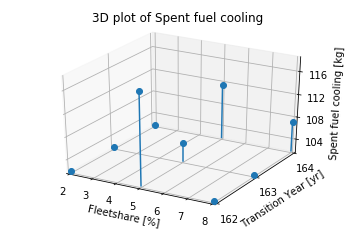
\includegraphics[width=0.4\linewidth]{figures/3d_sfc} 
        \caption{Inventory: Spent fuel cooling}
        \label{fig:3d_sfc}
    \end{subfigure}
    \begin{subfigure}[t]{0.4\textwidth}
        \centering
        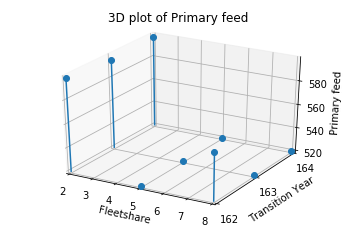
\includegraphics[width=\linewidth]{figures/3d_pf} 
        \caption{Inventory: Primary feed}
	    \label{fig:3d_pf}
    \end{subfigure}
    \begin{subfigure}[t]{0.4\textwidth}
        \centering
        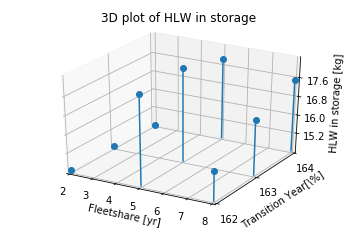
\includegraphics[width=\linewidth]{figures/3d_hlw} 
        \caption{Inventory: HLW in storage}
        \label{fig:3d_hlw}
    \end{subfigure}
    \caption{DYMOND EG01-30 Transition Scenario: ›Maximum amount of Pu [kg] in each inventory during each simulation for varying fleet share and transition start date.}
\end{figure}

Figures \ref{fig:3d_sfc}, \ref{fig:3d_pf}, and \ref{fig:3d_hlw}
communicate how fleet share ratio and introduction date of advanced 
reactor technology 
synergistically impact maximum Pu in various inventories in the 
\gls{NFC}. 
To better utilize this information for decision making, 
similar synergistic studies can be conducted for the output 
variables in all the evaluation metrics. 
The results from each study can be normalized, weighted, and 
combined to create an optimization surface similar 
to \ref{fig:passerini_payoff} to determine the ideal fleet share 
ratio and transition year combination. 

\subsubsection{\textbf{Cyclus}}
25 scenarios were evaluated for a combination of fleet share ratio 
of 0\%, 5\%, 10\%, 15\%, 20\% PWR MOX and advanced reactor introduction 
date of year 80 to 84.
Figures \ref{fig:cyclus_3d_hlw}, \ref{fig:cyclus_3d_depu}, and 
\ref{fig:cyclus_3d_ic}
visualize the final amount of HLW, final amount of depleted uranium, and
total amount of idle capacity in the scenario for varying 
fleet share and advanced reactor introduction date values. 

Figure \ref{fig:cyclus_3d_hlw} shows that for scenarios in which 
there is a smaller fleet share of \gls{MOX} \glspl{PWR}, and the 
transition begins later in the simulation, there is less high 
level waste produced. 
It is assumed that the initial \glspl{LWR} have a longer lifetime
and thus, advanced reactors exist in the simulation for a shorter 
amount of time, resulting in less reprocessing waste is produced. 
Also, \gls{MOX} \glspl{PWR} produce more \gls{HLW} than \glspl{SFR}. 
Figure \ref{fig:cyclus_3d_depu} shows that as the introduction date 
of advanced reactors is pushed back, more depleted uranium is produced 
due to extended lifetime of the \glspl{LWR} that utilize enriched 
natural uranium fuel that generates depleted uranium. 
Figure \ref{fig:cyclus_3d_ic} shows that idle capacity is minimized 
for a later advanced reactor introduction date. 
Having a later introduction date of advanced reactor technology ensures 
that a sufficiently large inventory of transuranic elements is amassed
to produce fuel for the \gls{MOX} \glspl{PWR} and \glspl{SFR}.  
This ensures that there is no gap in the supply chain that results 
in idle advanced reactor capacity.

% replace transition year 
\begin{figure}[]
    \centering
    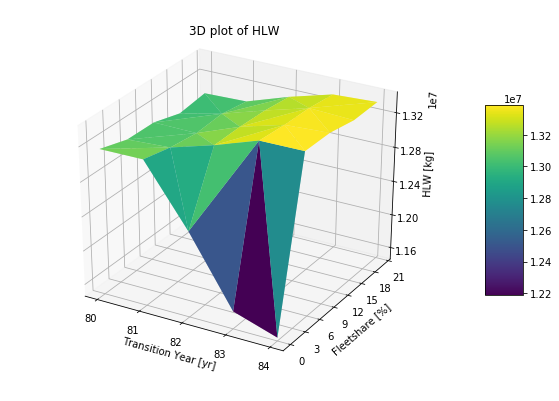
\includegraphics[width=0.7\linewidth]{cyclus_3d_hlw} 
    \caption{\Cyclus Transition Scenario: Final amount of HLW [kg] in the scenario during each simulation for varying fleet share and transition start date.}
    \label{fig:cyclus_3d_hlw}
\end{figure}

% replace transition year 
\begin{figure}[]
    \centering
    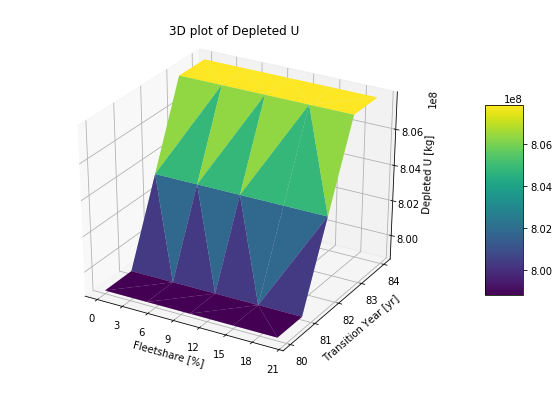
\includegraphics[width=0.7\linewidth]{cyclus_3d_depu} 
    \caption{\Cyclus Transition Scenario: Final amount of Depleted Uranium [kg] in the scenario during each simulation for varying fleet share and transition start date.}
    \label{fig:cyclus_3d_depu}
\end{figure}

% replace transition year 
\begin{figure}[]
    \centering
    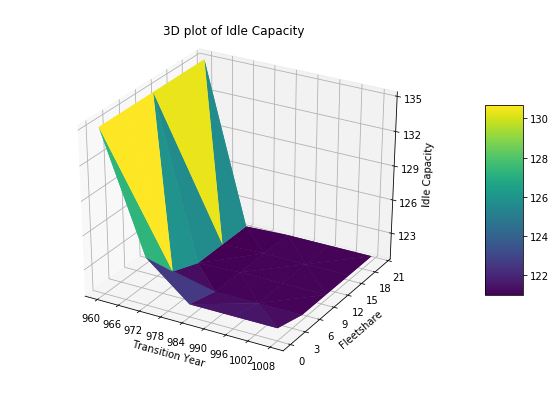
\includegraphics[width=0.7\linewidth]{cyclus_3d_ic} 
    \caption{\Cyclus Transition Scenario: Total amount of Idle Capacity [MW] in the scenario during each simulation for varying fleet share and transition start date.}
    \label{fig:cyclus_3d_ic}
\end{figure}

\section{Global Sensitivity Analysis}
\texttt{dcwrapper} was used to conduct a global sensitivity 
analysis study to generate Sobol indices which tells us which 
input parameters has the most influence on an output variable. 
This type of sensitivity analysis was described in 
section \ref{sec:sobol}. 
It is provides a more wholistic view of the system 
than OAT (section \ref{sec:oat}) and 
synergistic (section \ref{sec:synergistic}) sensitivity 
analysis, because it decomposes the variance of the 
output of the scenario simulation into fractions which can be 
attributed to each input, giving a better idea of the
most impactful input parameters. 
More than two variables could be varied in a synergistic
sensitivity analysis, but it is difficult to visualize the 
results. 

The input variables varied are: fleet share ratio, 
transition start year, and used fuel cooling time.
The output variables considered are final amount of HLW, 
final amount of depleted uranium, and total idle capacity. 
Table \ref{tab:sobol} provides the sobol indices that depicts 
the impact of variance of each input variable on each output 
variable. 
It provides a summary of the most influential input parameters 
are for each output parameter. 
Fleet share has the largest impact on 
final HLW value while transition start year has the largest 
impact on final depleted uranium value and the total idle 
capacity value in the simulation. 
Transition start year and cooling time have some influence on 
the final value of HLW. 
Fleet share and cooling time have no influence on the final 
depleted uranium value. 
    
    \begin{table}[H]
        \centering
        \caption{Sobol Indices for a global sensitivity analysis study of the impact of 
        fleet share \% of PWR MOX reactors, transition start year and cooling time on various output
        variables: final amount of HLW, final amout of depleted uranium, and total 
        idle capacity in the simulation}
        \label{tab:sobol}
            \scriptsize
            \begin{tabularx}{\textwidth}{L|LLL}
                \hline	
                \textbf{Input Variables}                      & \multicolumn{3}{c}{\textbf{Sobol Indices for Output Variables}}   \\ \hline
                & \textbf{Final HLW} & \textbf{Final depleted uranium} & \textbf{Total idle capacity} \\ \hline
                \textbf{Fleet Share} & 0.828     & 0                      & 0.00509             \\
                \textbf{Transition Year}                & 0.381     & 0.971                  & 1.505               \\
                \textbf{Cooling Time}                         & 0.126     & 0                      & 0                   \\ \hline

            \end{tabularx}
    \end{table}

\section{Main Takeaways}
\subsection{DYMOND Limitations}
For a transition scenario simulation in DYMOND, the user must 
manually edit the fuel management 
strategy to define which reactor the recycled 
part of each fuel type comes from for every year. 
This is found in the \textit{Source management} tab of a 
Dymond6 input file. 
Having the 
wrong fuel management strategy will result in idle reactor
capacity due to lack of fuel. 
Therefore, the user has to use trial and error to find a fuel 
management strategy to minimize or eliminate idle reactor capacity. 
With a 300-year simulation taking a few hours to run, it quickly 
becomes very tedious and time consuming.  

This issue impacted all sensitivity analysis analysis conducted 
with DYMOND because the fuel management strategy was 
optimized manually for certain scenario parameters, resulting in 
idle reactor capacity occurring when scenario parameters differed 
from it. 
To avoid this issue, an AI-based method (similar to \deploy) 
should be introduced to 
determine where the recycled part of each fuel comes from to 
minimize idle capacity in the simulation. 
This will ease the setting up of transition scenarios, and enable 
more effective and accurate sensitivity analysis studies.

\subsection{Importance of Different types of Sensitivity Analysis}
The OAT, synergistic, and global sensitivity analysis methods 
are all important for analyzing \gls{NFC} transition scenarios. 
Their use is in different forms. 
Global sensitivity analysis should be the first analysis conducted to 
determine which input variables are key to influencing the output 
variables of interest. 
OAT and synergistic sensitivity analysis can then be used together to 
do further analysis to determine the trends and quantitative impacts 
of specific input variables on specific output variables. 
